% !TeX encoding = UTF-8
% !TeX spellcheck = en_US

\documentclass[
	accentcolor=tud1a %Pick the color
]{tudreport}

% A couple of packages that may be useful
\usepackage{amsmath}
\usepackage{amsfonts}
\usepackage{amsthm}
\usepackage{algorithm2e}
\usepackage{listings}
\usepackage{xcolor}
\usepackage{tikz}
\usepackage{booktabs}
\usepackage[english]{babel}
\usepackage{blindtext}
\usepackage[caption=false,font=normalsize,labelfont=sf,textfont=sf]{subfig}
\usepackage{wrapfig}
\usepackage[hyphens]{url}


% Defining JavaScript listings
\definecolor{mygreen}{rgb}{0,0.3,0}
\definecolor{myyellow}{rgb}{0.3,0.3,0}
\definecolor{mygrey}{rgb}{0.9,0.9,0.9}

\lstdefinelanguage{JavaScript}{
  keywords={break, case, catch, continue, debugger, default, delete, do, else, false, finally, for, function, if, in, instanceof, new, null, return, switch, this, throw, true, try, typeof, var, void, while, with},
  morecomment=[l]{//},
  morecomment=[s]{/*}{*/},
  morestring=[b]',
  morestring=[b]",
  ndkeywords={class, export, boolean, throw, implements, import, this},
  keywordstyle=\color{blue}\bfseries,
  ndkeywordstyle=\color{darkgray}\bfseries,
  identifierstyle=\color{black},
  commentstyle=\color{purple}\ttfamily,
  stringstyle=\color{red}\ttfamily,
  sensitive=true
}

\lstset{
    frameround=fttt,
    language=JavaScript,
    numbers=left,
    breaklines=true,
    breakatwhitespace=true,
    keywordstyle=\color{blue}\bfseries, 
    basicstyle=\ttfamily\color{black},
    numberstyle=\color{black},
    stringstyle=\color{myyellow},
    commentstyle=\color{mygreen},
    backgroundcolor=\color{mygrey}
    }
\lstMakeShortInline[columns=fixed]|

%\begin{lstlisting}[float,caption=Code Example,label=l:code_example]
%var a;
%console.log(a);
%if(a) {
%	// This is a comment
%	console.log('Yeah');
%}
%\end{lstlisting}

\begin{document}
\title{ARSE: Agile Responsive Simple Environment}
\subtitle{Team Echo: Project Report for the course Internet Praktikum TK in WS 2015/16}
\subsubtitle{Elmi Faisal Ali \\
Enkhtuul Gankhuyag \\
Floriment Klinaku \\
Masaud Yakubu Alhassan \\
Omar Antonio Erminy Ugueto \\
Satia Herfert
}

\maketitle

\tableofcontents

\chapter{Introduction}
\label{ch:introduction}

Nowadays, agile development is usually complemented by an online tool to manage, collaborate and share the overall progress of a project. ARSE (Agile Responsive Simple Environment) is a web application that assists teams who use Scrum as a development methodology. 

ARSE offers the capability to manage projects with all the abstractions related to Scrum. After creating a project, the users of the application can define their product backlog. Furthermore, they can set the scope of a sprint in the form of a sprint backlog and, later on, the sprint can be started. 

The tool we introduce presents an interactive sprint board. Besides the standard functionalities of creating tasks and assigning user stories to project developers, the user updates the status of stories via a drag \& drop feature. This is one of the neat features that portrays how ARSE was developed considering user experience as an important factor.

ARSE was developed during the course TK Internet Praktikum in WS 2015/16 at TU Darmstadt. In the future, ARSE can be an open-source tool that teams all over the world could use and improve. 

The following report describes ARSE in both, its technical implementation as well as its use cases. The next section describes the architecture in technical terms. The user documentation describes the application in terms of the features that are offered to end-users. We conclude with the product backlog items that we included in ARSE as explained in the project specification. 


\chapter{Architecture}
\label{ch:architecture}

\begin{wrapfigure}{R}{0.5\textwidth}
  \centering
    \includegraphics[height=19EM]{img/architecture}
    \captionof{figure}{The architecture of ARSE}
    \label{fig:architecture}
\end{wrapfigure}
ARSE is built with the MEAN stack. The MEAN stack consists of \textbf{MongoDb}, \textbf{Express.js}, \textbf{Angular.js} and \textbf{Node.js}. Figure \ref{fig:architecture} illustrates the general architecture of an application built on top of the MEAN stack.

\begin{itemize}
\item \textbf{Node.js} is JavaScript runtime built on Chrome's V8 JavaScript engine. Node.js is used for building server side JavaScript web applications \cite{NJS}.
\item \textbf{Express.js} is web application framework for Node.js. It represents the backend of the application, handling aspects as API endpoints, controllers and database access via Mongoose (an object modelling mapper for MongoDb) \cite{EXJS}.
\item \textbf{MongoDb} is the database part of the application. It is a document oriented database where data is organized in JSON-like documents. MongoDb is particularly efficient when dealing with unstructured data \cite{MDB}.
\item \textbf{Angular.js} is a web application framework that provides client-side model-view-controller(MVC). Angular.js is the front end part of the application \cite{AJS}.

\end{itemize}

Figure \ref{fig:class-diagram} shows a class diagram of ARSE that explains the main entities used in the application as well as their relationships. In the next section explains the main responsibilities of each class. 

\begin{itemize}

\item \textbf{Project}: It represents the most important class in the application. The whole functionality of ARSE revolves around the creation and management of projects. A project has a name and a description that identify it. It contains a list of participants that can have access to the project's information; participants can execute different actions depending on their role in the project. A project belongs to a user that, by default, is the user that created it. Moreover, each project has a backlog that consists of a list of user stories. The backlog defines all the requirements of the product or service that is being built. During its lifetime, a project will have several sprints; a list of all past sprints is maintained as well as a reference to the current active sprint if any. Finally, each project has a private chat where all the participants can communicate.

Additionally, each project can maintain a list of additional story types and statuses that will be valid only for that project. These new configuration values can be added by the product owner of the project.

\item \textbf{Participant}: It represents an abstraction of a user inside the project. The product owner of a project can add or remove participants to a project with a particular role. The roles available are ``Product Owner'' and ``Developer''. A reference to the application user is kept in order to access identification attributes such as name and email.

\item \textbf{User}: It represents a user of the application. A new entry is created every time someone registers in ARSE. This class was modeled using the authentication framework of the ``AngularJS Full-stack Generator'' \cite{AFSG} and it serves as our main authentication and authorization mechanisms. It provides basic security features, as password encryption and session persistence via cookies.  

\item \textbf{Story}: It represents the user stories that belong to a project. User stories conform the building blocks of Scrum as they allow the product owner to guide the development process by prioritizing the features to be developed. A Story contains a brief summary and a detailed description, also, the estimated story points. During a sprint, stories undergo multiple status updates that indicate the development progress in that feature. A set of statuses is defined by default, however, the product owner can customize it to the team's needs by adding or removing statuses; this augmented list of statuses can only be used when the story is in the status ``In progress''. A similar situation occurs with the story types, although they can be set at any point. Moreover, a story can contain a list of tasks that breaks down the user story into particular activities. 

\item \textbf{Task}: It represent a detailed activity that is part of a user story. A tasks has no meaning by itself as it has to be associated with a user story. It contains a summary and a description of the activity to be done, as well as a status the describe its progress. However, the extended list of statues available in the project does not apply to tasks.

\item \textbf{Sprint}: It represents the execution and outcome of a sprint in the project. During its lifetime, a project will undergo multiple sprints. A sprint is defined by its starting date, its ending date and the total number of story points burnt. Some of these attributes might be empty if the sprint has not finished.

\item \textbf{Chat}: It represents the chat messages exchanged by the participants of a project. Every message is stored so it could be browsed again later on. A chat message is defined by the user who posted it, the text content of the message and the date when it was sent.

\end{itemize}

\begin{wrapfigure}{H}{\textwidth}
  \centering
    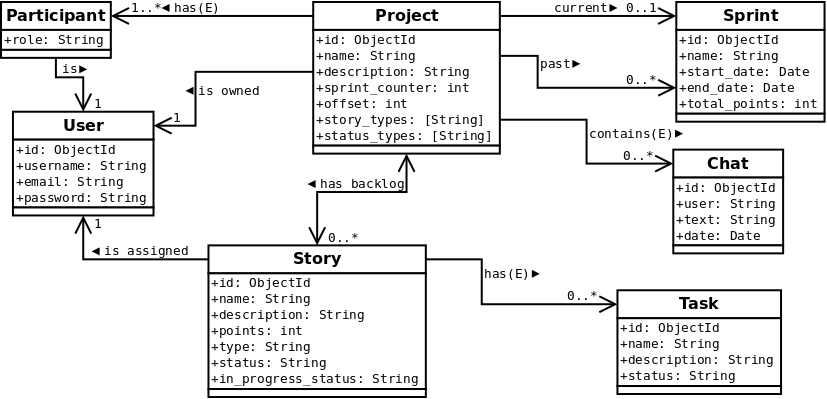
\includegraphics[height=20EM]{img/class-diagram}
    \captionof{figure}{Class Diagram. Relationships marked with an ``(E)'' indicate that the information of the incoming class is embedded in the outgoing class. The remaining relationships are reference-based.}
    \label{fig:class-diagram}
\end{wrapfigure}

% TODO Add additional interesting features
% Use of embedded objects
% Use of middleware in express
% Use Angular directives
% Use of socket.io
% Use of bootstrap and css preprocessors (mention also responsiveness)

\chapter{User Documentation}
\label{ch:use-documentation}

In this chapter we will briefly explain how to use the main features of our application. For each state or thematic group of use cases, we present a section that explains the graphical layout and the possible ways to interact with the tool.

\section{Profile Management}
\label{sec:profile-mgmt}
%Explain: Register, Login, Logout, change Profile

\begin{wrapfigure}{R}{0.5\textwidth}
  	\centering
	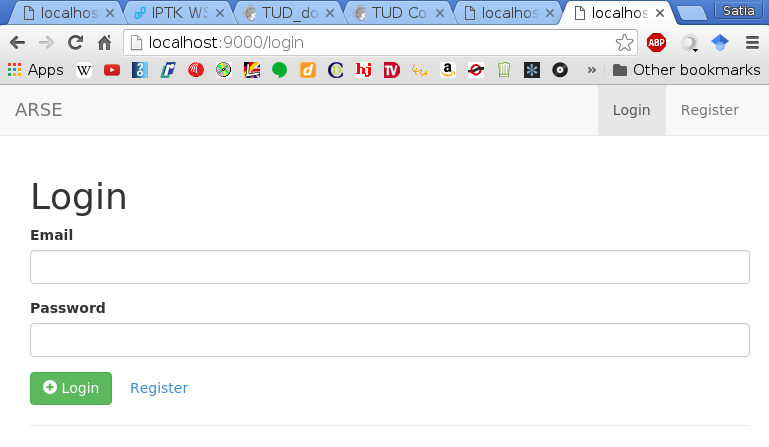
\includegraphics[width=0.48\textwidth]{img/login}
	\caption{The login screen.}
	\label{fig:login}
\end{wrapfigure}

When first visiting ARSE, you will be asked to login or register. The screen you will see is displayed in figure \ref{fig:login}. Here you can input the right information to login (1) or click \emph{Register} (2) to switch to a different form where you are asked to register providing your full name, email address and a password. Email addresses serve as usernames and must be unique in the system.

\section{Project Management}
\label{sec:project-mgmt}
%Explain: List of projects, create project, modify/delete project.

\begin{wrapfigure}{R}{0.5\textwidth}
	\centering
	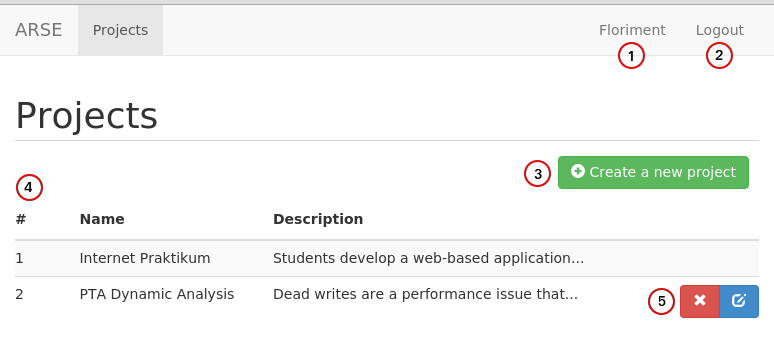
\includegraphics[width=0.48\textwidth]{img/projects}
	\caption{The project list screen.}
	\label{fig:project-list}
\end{wrapfigure}

After logging in, you will be redirected to a page that shows the projects you are a member of, as depicted in figure \ref{fig:project-list}. You can click on your name in the upper right corner of the navigation bar in order to access a page that allows you to edit your profile (1). In that page you can adjust your name and password, but not your email address. The email address cannot be changed after the registration. Changes to your profile always require a password confirmation using your current password. In the upper right corner you will also find a button that logs you out from the system (2).

If you just registered in the application, the projects page will be empty. You can now create your own projects or ask colleagues to add you to their projects.

In order to create a project, click the button \emph{Create a new project} (3). This will open a form where you need to fill out name and description of the project. After that, the project will appear in the list (4) and you will automatically become product owner of this project. This gives you privileges that normal developers in a project do not have.

The projects are listed with name and description. If you are product owner of a project, some control buttons will be available (5); you can use them to delete or modify a project.

%Explain: Project-navbar
You can click the name of a project in the list to access the project page. When you click it, you are redirected to a project specific space, which includes a navigation bar to access the different views available for each project. On the left-hand side of figure \ref{fig:project-backlog}, the project navigation bar is displayed (1). On mobile devices, this navigation bar is displayed at the top instead. It includes five icons that trigger different project-related views. Each view is explained in detail in the following subsections.
\begin{description}
	\item[Product Backlog:] A list of all stories of the project can be viewed here. Stories can be added, removed and edited. Furthermore, it is possible to start a new sprint in this view.
	\item[Sprint Board:] This view can only be accessed if a sprint is currently running. Its purpose is to allow changing the status of stories, managing the tasks of stories, or to close or cancel a sprint.
	\item[User management:] The participants of the project are displayed in this view. As a product owner, it is also possible to add or remove members as well as to change their roles in the project.
	\item[Past Sprints:] This view simply lists all finished sprints, with their time-frames and the number of story points that were burnt in the sprint.
	\item[Project configuration:] This view is only accessible by product owners; the icon will be hidden for developers. The view allows you to define additional story types and statuses. These can then be used on every story of the project later on.
\end{description}


\subsection{Product Backlog}
\label{sec:backlog}

%Explain: Adding items, viewing/modifying/deleting items, reordering items, dragging sprint delimiter, starting sprint.

\begin{wrapfigure}{R}{0.5\textwidth}
	\centering
	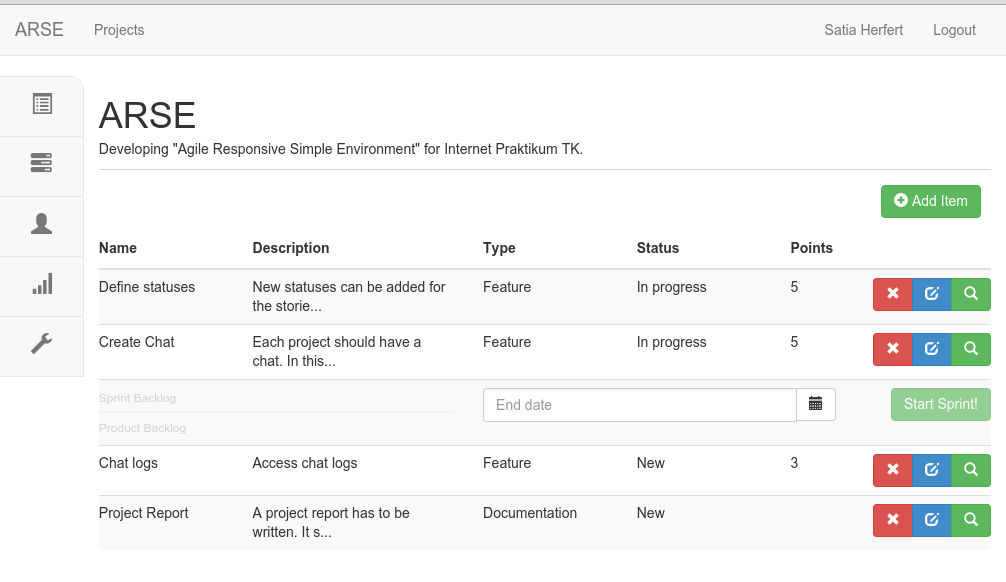
\includegraphics[width=0.48\textwidth]{img/backlog}
	\caption{The project backlog screen with the project navigation bar on the left-hand side.}
	\label{fig:project-backlog}
\end{wrapfigure}

This view lists all stories of a project, in priority order (2). An example of how this can look is given in figure \ref{fig:project-backlog}. For each story, name, description, type, status and story points are given. Three buttons follow in each row of the table (3). The first two allow to delete or modify a story; the last displays more details about the story on the left side of the screen.

In the top there is a button that can be used to add a new story (4). The required information is a name and a description, the number of story points, the story type and the assignee. It is possible to leave a story without an assignee. The form shown has the same layout as when editing stories.

To change the order --and thereby the priority-- of stories, users can simply drag and drop the rows up or down in the table. There is one special row that is always present: the sprint delimiter (5). In the example screenshot, this is the third row. This delimiter separates the sprint backlog (above) from the product backlog (below). It can be dragged like any other row, effectively changing the scope of a sprint. This will issue a warning, if a sprint is currently active. The sprint backlog is the subset of all stories that are expected to be done by the end of the sprint.

Finally, in the row of the sprint delimiter, product owners have the possibility to start a new sprint. In order to that, first the planned end date has to be chosen and afterwards the button \emph{Start Sprint!} can be clicked (6).

\subsection{Sprint Board}
\label{sec:sprint-board}

%Explain: Cancelling sprint, closing sprint, dragging stories, viewing stories, assigning a team member, adding tasks, changing tasks, dragging tasks, collapse/expand to view tasks, colors, selecting tag/status.

This view becomes available after a sprint has been started. Given the big difference in screen sizes, the view is designed differently for desktop and mobile versions. In the following, first the desktop version is explained with all available features, and then the key differences to the mobile version are pointed out. An example of the desktop version is given in figure \ref{fig:project-sprintboard-desktop}, and for the mobile version in figure \ref{fig:project-sprintboard-mobile}.

\paragraph{Desktop version}
In the top there are two buttons displayed for product owners. They can be used to cancel or close a sprint respectively (1). Canceling means that all stories are transferred back to product backlog, regardless of their status. When closing a sprint, only the stories not done are transferred back; the finished stories are deleted. Please note that this action is irreversible and data may be lost if clicking this by accident.

Below that, there is a table that resembles a physical sprint board in agile projects (2). There are three columns, for new, started, and finished stories. Each story has its own row in the table and is displayed in a colored card providing essential information about it (3). The cards can be dragged and dropped into other columns to change the status of the story.

The color of the card and the upper left icon are chosen according to the its type. In addition, you can see the name of the story, and the associated story points. The plus icon allows to add tasks to the story, which are explained below. The magnifying glass shows all details of the story on the right-hand side of the screen, in the same way as in the product backlog view. The person assigned to a story is displayed in a second line on each card, and it can also be changed in-place. Moreover, stories that are in progress (second column), allow to have an additional status assigned. This is a tag that can be used if the three statuses do not suffice. Product owners can configure these tags in the project configuration. This modifiable tag is displayed in a third line, if tags have been defined.

If tasks have been added to a story, they are displayed in gray cards below the story with title and description (4). Just as stories, they can be dragged to other columns to change their statuses. These gray cards also have icons to edit or delete the task. To show or hide the tasks of a story, the arrow pointing down or up on the story card can be clicked.

\paragraph{Mobile version}

On the small screens of mobile devices it is not possible to show all three columns simultaneously Therefore, the table has been replaced by a set of three tabs for the respective statuses (5). Now, all information is displayed on the cards, including the description, and no magnifying glass icon is available. To change the status of a story or task, right and left arrow icons have been added (6). Tasks are always displayed in the mobile version and cannot be hidden as in the desktop version. As it is possible that a task is in a different tab as the story it belongs to (for example the task \emph{Browsing} in figure \ref{fig:project-sprintboard}), the name of the story is always displayed in the upper right corner of a task card. The controls to change assignees or tags, and the buttons to close or cancel a sprint have not been changed.

\begin{figure}[ht]
\centering
\subfloat[]{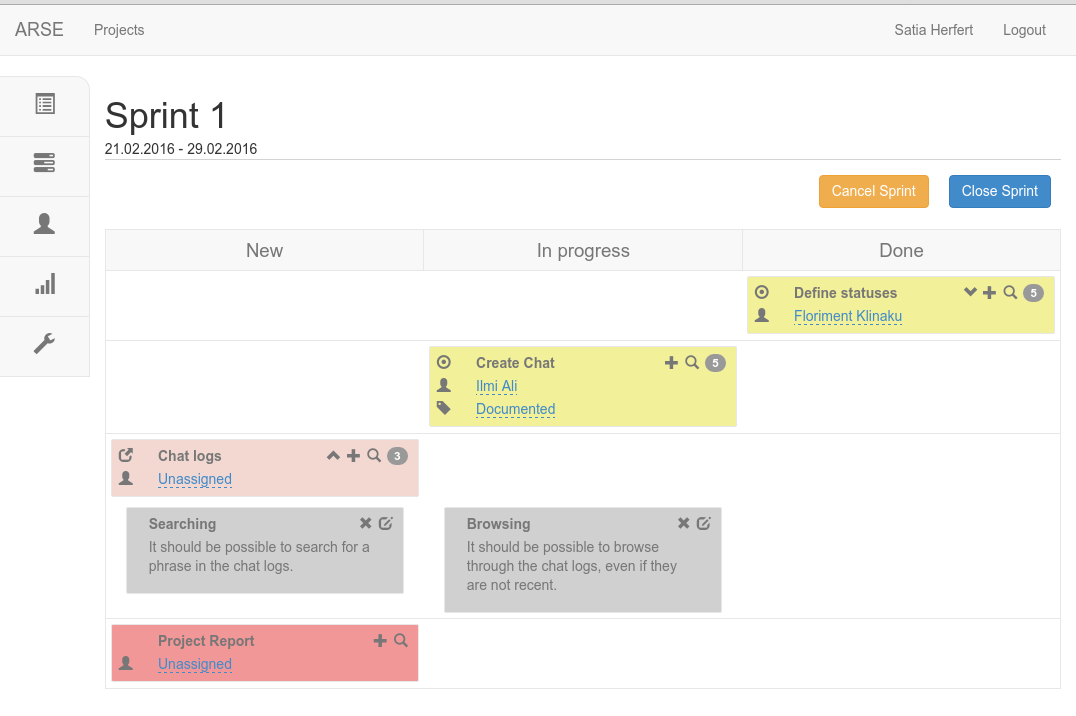
\includegraphics[height=20EM]{img/sprintboard}%
\label{fig:project-sprintboard-desktop}}
\hfil
\subfloat[]{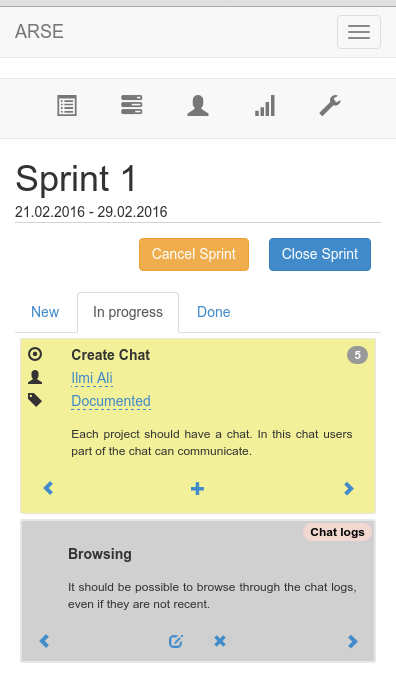
\includegraphics[height=20EM]{img/sprintboard-mobile}%
\label{fig:project-sprintboard-mobile}}
\caption{The sprint board in its desktop and mobile versions.}
\label{fig:project-sprintboard}
\end{figure}

\subsection{User Management}
\label{sec:user-mgmt}

The user management view, depicted in Figure \ref{fig:project-user-management}, lists all participants of the project. All developers can see the names, email addresses and roles of their project colleagues. As a product owner, it is also possible to change the role of other participants, or to remove users from the project (1).

Product owners also see another set of controls below, that allows them to add new participants to the project (2). A text field can be used to search for usernames or email addresses. By clicking the corresponding row in the search results, a user is chosen to be added. Finally, the role of the new user can be chosen between \emph{Developer} and \emph{PO} (product owner), before clicking the \emph{Add user} button.

\begin{figure}[ht]
\centering
\begin{minipage}{.5\textwidth}
  \centering
  	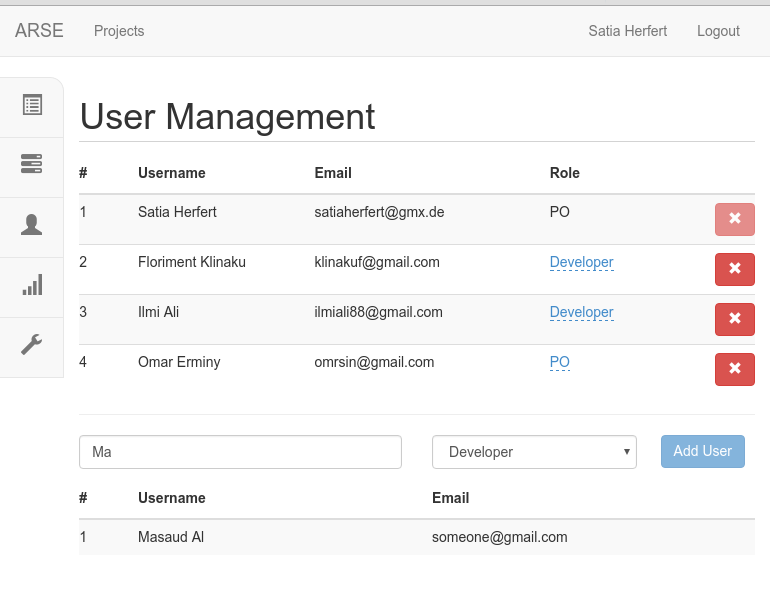
\includegraphics[height=15EM]{img/usermgmt}
  	\captionof{figure}{The user management of a project.}
  	\label{fig:project-user-management}
\end{minipage}%
\begin{minipage}{.5\textwidth}
	\centering
	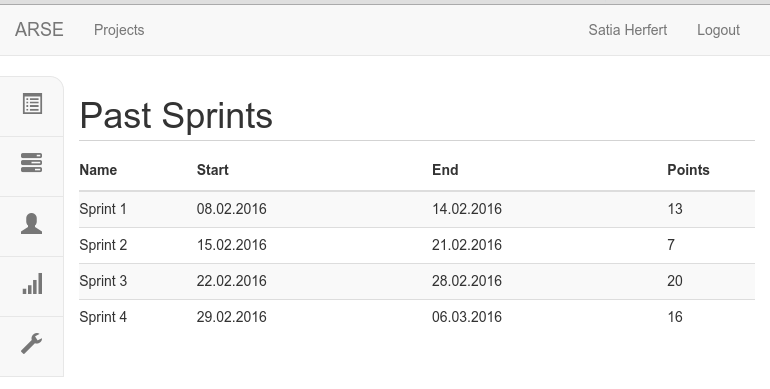
\includegraphics[height=15EM]{img/pastsprints}
	\captionof{figure}{The past sprints of a project.}
	\label{fig:project-past-sprints}
\end{minipage}
\end{figure}

\subsection{Past Sprints}
\label{sec:past-spints}

%Explain: Table of past sprints

This view is solely informative and does not contain any controls; an example can be seen in figure \ref{fig:project-past-sprints}. A table lists all past sprints with their respective start and end dates, and the amount of story points that were burned in the sprint. This is the sum of the story points of stories that were finished in the sprint.

\subsection{Project Configuration}
\label{sec:proj-config}

%Explain: Adding story types, removing story types, adding statuses, removing statuses

The project configuration view is only accessible by product owners; it is depicted in \ref{fig:project-config}. It has two purposes: managing story types and additional statuses (tags) of stories. For both, a list of the currently defined items is shown, and a button to remove a story type or status (1)(2). The first table also displays the colors of the story types that are used in the sprint board (3). Moreover, there are text fields and buttons to add new types or statuses (4)(5). 
\begin{figure}[ht]
\centering
\begin{minipage}{.5\textwidth}
  \centering
	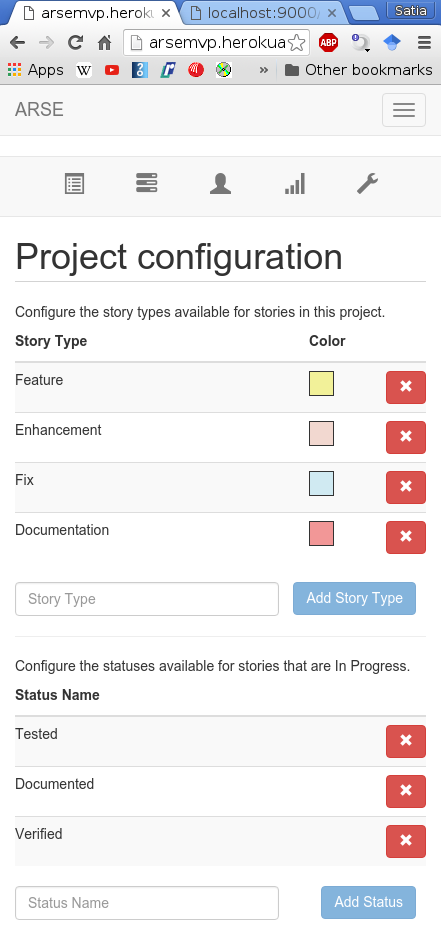
\includegraphics[height=28EM]{img/configuration}
	\caption{The project configuration.}
	\label{fig:project-config}
\end{minipage}%
\begin{minipage}{.5\textwidth}
	\centering
	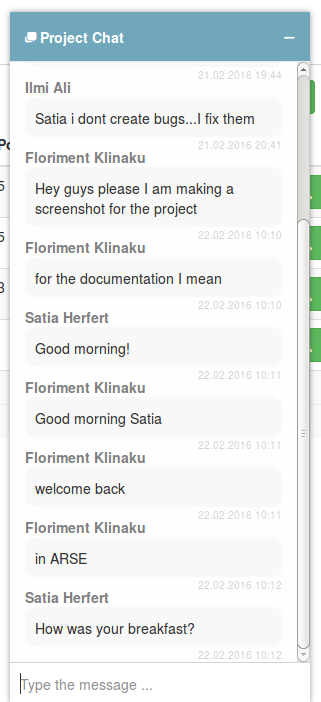
\includegraphics[height=28EM]{img/chat}
	\caption{The Chat Window.}
	\label{fig:chat}
\end{minipage}
\begin{minipage}{.5\textwidth}
	\centering
	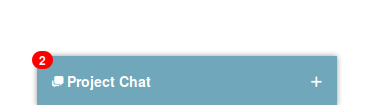
\includegraphics[width=0.6\textwidth]{img/chatNotification}
	\caption{The Chat Window minimized.}
	\label{fig:chat-notification}
\end{minipage}
\end{figure}

\subsection{Chat}
\label{sec:chat}
ARSE also offers a group chat. Each project has its own group chat, where members of that specific project can discuss about issues relevant to that space. The chat is displayed in the bottom-right corner and it is shown in each view of the project (e.g. Sprint Board, Backlog, ...). The chat window is collapsible, it can be in two different states: shown (Figure \ref{fig:chat}) and minimized or hidden (Figure \ref{fig:chat-notification}). 

When the chat window is minimized, each time a new message arrives there is a red indicator displaying the number of new unseen messages. When displayed, it shows the 10 most recent messages, offering also the possibility to search through older messages by clicking the ``Load more'' button which appears on top of these messages. By clicking the button, 10 more messages are loaded. The chat is also mobile-friendly, where in the same corner a floating action button appears. Through this button the chat window can be collapsed and minimized. The messages exchanged per project are persistent. 


\chapter{Done Product Backlog Items}
\label{ch:done-pbis}

In the following we list all the items from the original product backlog that were developed in this project. Certain stories have been moved to make the actions available to a different class of users, so that the product is more compatible with the idea of Scrum. The roles in our project are users, registered users, team members (of a project), and product owners (of a project). This list also contains stories that were modified or added to the original backlog.

%TODO go through our modified backlog and see if we need to add more stories here.

\begin{itemize}
	\item As a user, I can
	\begin{itemize}
		\item register to the system with user name, email and password. (Unique usernames)
		\begin{itemize}
			\item Users can be assigned to different projects with different roles.
		\end{itemize}
		\item access the web application with different kinds of devices (mobile, tablet, pc ...).
	\end{itemize}
	
	\item As a registered user, I can
	\begin{itemize}
		\item edit my profile (name, password).
		\item see the list of projects I am a member of.
		\item create new projects (name and description), and become automatically the product owner of these projects.
	\end{itemize}

	\item  As a team member of a project, I can
	\begin{itemize}
		\item access the Product Backlog.
		\item access the Sprint Board.
		\item access past sprints which includes their name, time interval, and story points burnt.
		\item copy backlog items to the Sprint Backlog.
		\item create new tasks in the Sprint Board (a task always belongs to a user story).
		\item change product backlog items including their description as well as their status (New, in progress, done).
		\item change tasks including their description as well as their status (New, in progress, done),
		\item assign product backlog items to a team member.
		\item add new product backlog items to the product backlog of a project.
		\begin{itemize}
			\item product backlog items can have different statuses (new, in progress, done).
			\item product backlog items can be of different types, e.g. feature, enhancement, fix.
		\end{itemize}
		\item change the order (priority) of product backlog items in the product backlog.
		%\item chat with my team members
		%\item access and search chat logs
	\end{itemize}
	
	\item As a product owner of a project, I can
	\begin{itemize}
		\item create a new Sprint (a new Sprint cannot be created if there's one already running) with name, description, time-box and initial Sprint Backlog.
		\item assign registered users to a project.
		\item assign roles to project members (team member, product owner).
		\item change the list of statuses assignable to product backlog items in the project settings.
		\item change the list of types assignable to product backlog items in the project settings.
		\item close a Sprint (all done stories will be removed).
		\item cancel a Sprint.
	\end{itemize}
\end{itemize}

%TODO Include a list of undone stories (if we have any)
%Bonus features
%users must confirm their registration by clicking on a registration link sent via email
%feature of burntdown charts
%use special interaction features with mobile devices like shaking

\bibliographystyle{abbrvnat}
\bibliography{references}
\end{document}
